% ==================================================================
% 1. Introduction   (file: sections/03_introduction.tex)
% ==================================================================
\section{Introduction}
\label{sec:intro}

\begin{figure}[t]
\centering
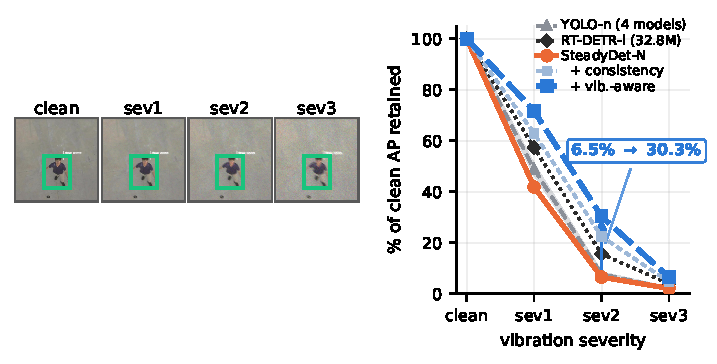
\includegraphics[width=0.95\textwidth]{figures/fig1_teaser.pdf}
\caption{\textbf{Compact aerial detectors go blind when the airframe vibrates.}
A flight frame under each VisDrone-Shake severity (sev1 and sev2 are ordinary flight,
not a fault), and the fraction of clean AP that survives on VisDrone-person, over
three seeds. Every published detector collapses at the same rate: the failure
belongs to the regime, not to one network.}
\label{fig:teaser}
\end{figure}

A detector that scores well on an aerial benchmark can still be unusable on an
actual aircraft, for a physical reason the literature largely ignores: a
multirotor vibrates. Rotor imbalance, motor harmonics and frame resonance
transmit high-frequency motion to the camera, and because the sensor integrates
over a finite exposure, that motion appears as directional blur, elevated noise
and frame-to-frame brightness oscillation. Unlike weather or occlusion this
corruption is not occasional; it is present whenever the rotors are spinning.

We began by measuring how much it matters, on our own detector first. SteadyDet-N
is an anchor-free network of $1.17$\,M parameters and $4.6$ GFLOPs built for
tiny-person detection from a UAV, and under a four-level vibration model it falls
from $0.189$ to $0.012$ average precision at moderate severity, retaining
$16.8 \pm 0.7\%$ of its clean accuracy. Fig.~\ref{fig:teaser} shows the collapse is
not ours alone: every published detector we measured falls at the same rate. A
detector blind whenever the aircraft is airborne is not a detector, and on this
axis the entire compact-detection literature is in the same position.

The obvious responses are unattractive on a small UAV. Isolation and gimbals cost
mass, payload and power; deblurring adds a second network to a pipeline that must
already fit a detector, a tracker and a controller into a $50$\,ms budget on a
passively cooled board. Every one pays at run time, on the platform least able to
afford it.

The response we test is deliberately blunt: put the vibration into the training
distribution. Each batch is replaced, with probability one half, by a corrupted copy
drawn from a physically motivated model of rotor-induced degradation, and the
ordinary detection loss is computed on whatever the network receives. Because blur,
noise and brightness scaling do not move objects, the labels remain valid and
nothing else changes. At inference the corruption does not exist and the exported
network is identical to the baseline, so the robustness costs nothing where cost is
felt.

Neither the network nor the regime suffices alone, and we show this rather than
assert it. Untreated, SteadyDet-N is the least accurate row in our table under
vibration; applied to YOLO11-n, the identical regime changes nothing at all, from
COCO weights or from scratch. Only the combination moves, and it moves past all
four YOLO nano variants while remaining the smallest and cheapest network compared.
That null result is also what keeps the comparison fair: our treated detector is
measured against a baseline that cannot be improved the same way, not against a
handicapped one.

We also tried something more elaborate, a consistency formulation, and report that
it is measurably worse at $1.8\times$ the training cost. A control contradicting the
authors' expectation is worth more to a reader than one confirming it.

Our contributions are: \textbf{(i)} \emph{SteadyDet-N with its training regime},
which at $1.17$\,M parameters and $4.6$ GFLOPs loses to every YOLO nano variant on
clean VisDrone and leads all of them on accuracy under vibration, exceeding
RT-DETR-l at $28\times$ its size at the severity of ordinary forward flight
(Section~\ref{sec:baselines}); \textbf{(ii)} \emph{VisDrone-Shake}, a seeded
four-level vibration protocol under which every detector we tested loses
$74$ to $83\%$ of its average precision (Sections~\ref{sec:shake}
and~\ref{sec:baselines}); \textbf{(iii)} \emph{vibration-aware training}, raising
retention from $16.8 \pm 0.7\%$ to $36.2 \pm 0.7\%$ at zero inference cost, with
the control showing the $120$ additional epochs contribute nothing on their own
($16.9 \pm 0.7\%$) (Section~\ref{sec:mainresults}); \textbf{(iv)} a controlled
negative result, that the consistency formulation we expected to be better is
measurably worse while costing more to train (Section~\ref{sec:mainresults}); and
\textbf{(v)} evidence that the architecture and the regime are each necessary,
since the same regime applied to YOLO11-n produces no effect at all and three
candidate explanations for that are tested and rejected
(Section~\ref{sec:generality}).
